\begin{problema}\leavevmode
\begin{enumerate}[label=\textbf{\alph*)}]
\item Los pesos correspondientes son

\begin{align*}
w_0 &= \int_{a}^{b} \frac{\left(x - \frac{a+b}{2}\right)(x - b)}{\left(a - \frac{a+b}{2}\right)(a - b)} \, dx
\end{align*}

Tomando el cambio de variable \( x = \frac{b-a}{2}t + \frac{a+b}{2} \), se tiene \( dx = \frac{b-a}{2} \, dt \) y

\begin{align*}
w_0 &= \int_{-1}^{1} \frac{\left(\frac{b-a}{2}t\right) \left(\frac{b-a}{2}t + \frac{a-b}{2}\right)}{\left(\frac{a-b}{2}\right)(a-b)} \frac{b-a}{2} \, dt \\[1em]
&= \frac{b-a}{4} \int_{-1}^{1} \frac{(b-a)^2\ t(t-1)}{(a-b)^2} \, dt \\[1em]
&= \frac{b-a}{4} \int_{-1}^{1} (t^2 - t) \, dt \\[1em]
&= \frac{b-a}{4} \left[ \frac{1}{3}t^3 - \frac{1}{2}t^2 \right]_{-1}^{1} \\[1em]
&= \frac{b-a}{4} \times \frac{2}{3} \\[1em]
&= \frac{b-a}{6}
\end{align*}


\begin{align*}
w_1 &= \int_{a}^{b} \frac{(x - a)(x - b)}{\left(\frac{a+b}{2} - a\right)\left(\frac{a+b}{2} - b\right)} \, dx \\[1em]
\end{align*}

Tomando nuevamente el cambio de variable \( x = \frac{b-a}{2}t + \frac{a+b}{2} \), se tiene:

\begin{align*}
w_1 &= \int_{-1}^{1} \frac{\left( \frac{b-a}{2}t + \frac{b-a}{2} \right) \left( \frac{b-a}{2}t + \frac{a-b}{2} \right)}{\left( \frac{b-a}{2} \right) \left( \frac{a-b}{2} \right)} \frac{b-a}{2} \, dt \\[1em]
&= \frac{b-a}{2} \int_{-1}^{1} (t + 1)(-t + 1) \, dt \\[1em]
&= \frac{b-a}{2} \int_{-1}^{1} 1 - t^2 \, dt \\[1em]
&= \frac{b-a}{2} \left[ t - \frac{1}{3}t^3 \right]_{-1}^{1} \\[1em]
&= \frac{b-a}{2} \times \frac{4}{3} \\[1em]
&= \frac{4}{6}(b - a)
\end{align*}

Para el peso \(w_2\) notemos que el polinomio cuadrático sobre el cual integramos es exactamente el mismo que para el peso $w_1$ pero trasladado \(\dfrac{a+b}{2}\) unidades hacia la derecha, y ambos casos integramos sobre un intervalo de longitud \(\dfrac{a+b}{2}\), por lo tanto \[w_2=w_1=\frac{b-a}{6}\]

\item\leavevmode Debido a que la función sobre la cual integramos, es un polinomio cubico cuyas tres raíces reales estan uniformemente espaciadas, resulta ser una función que es simetrica respecto al punto $(\frac{a+b}{2},\ 0)$, podemos decir que es una función impar respecto a la recta $x=\frac{a+b}{2}$, y entonces, al integrar sobre el intervalo $[a,\ b]$, la integral se anula, debido a que las áreas se cancelan.
\begin{figure}[h]
    \centering
    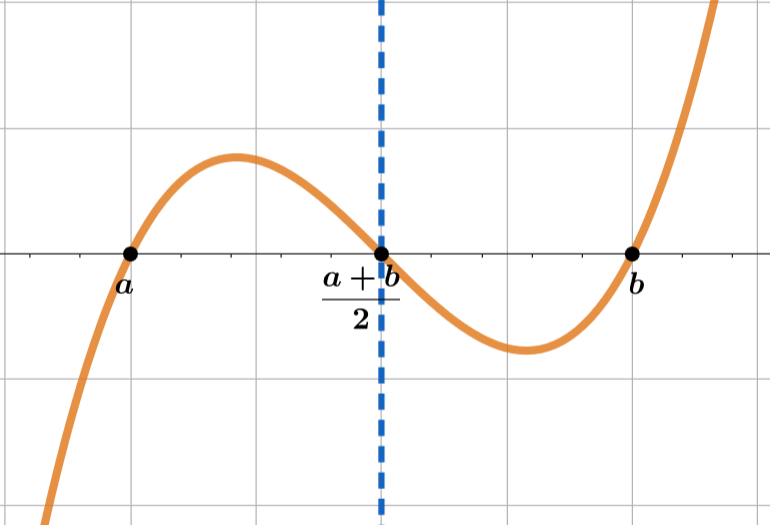
\includegraphics[width=0.5\textwidth]{img/tarea9_2c.png}
\end{figure}
\item  \leavevmode
\begin{enumerate}[leftmargin=1cm, labelsep=-1cm, itemindent=1cm]
    \item[Regla del trapecio]\leavevmode
    
    \begin{align*}
        \int_0^\pi \sin(x) dx &\approx \frac{\pi}{2}\left[\sin(\pi)+\sin(0)\right]=0
    \end{align*}

    \item[Regla de Simpson]
    \begin{align*}
         \int_0^\pi \sin(x) dx &\approx \frac{\pi}{6}\left[\sin(\pi)+4\sin\left(\frac{\pi}{2}\right)\sin(0)\right]\\[1em]
         &=\frac{2\pi}{3}\\[1em]
         &\approx 2.094
    \end{align*}
\end{enumerate}

Dado que una antiderivada para $\sin(x)$ es $-\cos(x)$ podemos evaluar explícitamente la integral anterior
\begin{align*}
    \ \int_0^\pi \sin(x) dx = -\cos(\pi)+\cos(0)=2
\end{align*}

Analizando los resultados, podemos notar que la regla de Simpson da una muy buena aproximación al valor real de la integral, mientras que la regla del trapecio dista de ser un método adecuado, esto debido a que $\sin(\pi)=\sin(0)=0$, por lo que resultaría más adecuado usar la regla del trapecio compuesta sobre un mayor número de puntos.

\end{enumerate}
\end{problema}